\mode<all>
% Incluyo los paquetes necesarios.
% para no tener problemas con acentos etc.
\usepackage[utf8]{inputenc}
% en español
\usepackage[spanish]{babel}
%matemática
\usepackage{amsmath}
% este no se si hace falta pero por las dudas
\usepackage{graphicx}
% para incluir peliculas
\usepackage{multimedia}
% para usar segunda pantalla
\usepackage{pgfpages}
\usepackage{pgf}
% para hacer dibujitos
\usepackage{tikz}
\usetikzlibrary[automata,calc,arrows,decorations.pathmorphing,backgrounds,
patterns,positioning,fit,petri,overlay-beamer-styles]
\tikzstyle{every picture}+=[remember picture]
%recuadros sencillos
%\usepackage{tcolorbox}
% enumeradores intercambiables
\usepackage{enumerate}
% para subtitulos en figuras
\usepackage{subcaption}
\definecolor{codegreen}{rgb}{0,0.6,0}
\definecolor{codegray}{rgb}{0.5,0.5,0.5}
\definecolor{codepurple}{rgb}{0.58,0,0.82}
\usepackage{listings}
\lstset{
    basicstyle=\fontsize{6}{8}\selectfont\ttfamily, 
    backgroundcolor=\color{Beige},   
    frame=lines,
    commentstyle=\color{codegreen},
    keywordstyle=\color{magenta},
    numberstyle=\tiny\color{codegray},
    stringstyle=\color{codepurple},
    breakatwhitespace=false,         
    breaklines=true,                 
    captionpos=b,                    
    keepspaces=true,                 
    numbers=left,                    
    numbersep=5pt,                  
    showspaces=false,                
    showstringspaces=false,
    showtabs=false,                  
    tabsize=4
}
%verbatim input from file!
\usepackage{verbatim}
% para modificar los encabezados y pies de página.
%\usepackage{fancyhdr}
%\pagestyle{fancy}
\usepackage{standalone}

%\mode<presentation>{
% para ver las notas con la presentacion.  
%\setbeameroption{hide notes}
%para dejar las notas en la segunda patnalla
%}

% incluyo los beamercolors
%%%%%%%%%% BEAMERCOLORS
% el recuadro para el titulo
\setbeamercolor{title}{fg=white,bg=Purple}
% el recuadro para el subtitulo
\setbeamercolor{subtitle}{fg=white,bg=DarkOliveGreen}
% los títulos de las secciones tienen su colorinche:
\setbeamercolor{sectionbox}{fg=white,bg=Purple}
% cada diapositiva tendrá su color de título.
\setbeamercolor{frametitle}{fg=white,bg=ForestGreen}
% el título de las secciones tienen también su color. 
\setbeamercolor{sectiontitle}{fg=white,bg=violet}

%%%% CUSTOM BEAMERCOLORS
% estos cuadros los defino para ubicar al lector en los temas que se tratan
% son los cuadritos que aparecen arriba del título. 
\setbeamercolor{structure0}{fg=white,bg=gray}
\setbeamercolor{structure1}{fg=black,bg=DarkGray}
\setbeamercolor{structure2}{fg=black,bg=lightgray}
% defino un cuadro para usar en alguna oportunidad, creo que para titulos. 
\setbeamercolor{whitebox}{fg=black,bg=white}
% un cuadro para resaltar
\setbeamercolor{highlight1}{fg=black,bg=Gold}

% beamer colors for headers and etc.
\setbeamercolor{header1}{fg=white,bg=Blue}
\setbeamercolor{header2}{fg=black,bg=Red}
\setbeamercolor{header3}{fg=black,bg=ForestGreen}

%code block
\setbeamercolor{codeblock}{fg=Blue, bg=Beige}
\setbeamerfont{codeblock}{family=\ttfamily,size=\scriptsize}


%incluyo el tema y modificaciones
%%% BEAMER THEME
% el tema 'boxes' es igual al default pero permite definir boxes de estructura 
% a mano. 
\mode<presentation>{
  \usetheme{boxes}
  % los boxes que identifican lo que se esta leyendo
    % box de la izquierda: la materia (subtitulo)
    \addheadbox{structure2}{\quad \tiny \insertshortsubtitle}
  %  box del medio en cabecera, el titulo de la clase
    \addheadbox{structure0}{\quad \tiny  \insertshorttitle \quad } 
  % box en a la derecha , eltítulo de la sección. 
    \addheadbox{structure1}{\quad \tiny \insertsection}
}
% tema interno y de colores para las diapositivas normales. 
\useinnertheme{rectangles}
\usecolortheme{dove}
% la fuente de las ecuaciones
\usefonttheme[onlymath]{serif}

% entorno codeblock para meter piezas de código.
% el color se definió en BEAMERCOLORS

\newenvironment{codeblock}
{
  \begin{beamercolorbox}{codeblock}
    \usebeamerfont{codeblock}
}
{
  \end{beamercolorbox}
}



% modifico los temas
  \titlegraphic{\includegraphics[width=0.25\textwidth]{./PREAMBLE/logo-isabt25.png}
  		\hfill
		\includegraphics[width=0.25\textwidth]{./PREAMBLE/ISOLOGOCNEA.png}
		\hfill
  		\includegraphics[width=0.25\textwidth]{./PREAMBLE/unsam-horizontal.png}}

\mode<presentation>{
\setbeamertemplate{title page}[center]
{
  %\includegraphics[width=0.25\textwidth]{./PREAMBLE/ISOLOGOCNEA.png}
  \inserttitle
  \insertsubtitle
  \insertauthor
  \insertinstitute
%  \inserttitlegraphic
}
}


% defino el template para las dapositivas con los titulos de las secciones. 
%es una recetita que saqué de algun lado. 
\setbeamertemplate{section page}{
  \begin{beamercolorbox}[ht=5ex,dp=1ex,wd=\paperwidth,center]{sectionbox}
    \begin{centering}
     \usebeamerfont{section  title} \insertsection 
    \end{centering}
  \end{beamercolorbox}
}
\AtBeginSection[]{
  \begin{frame}[plain]
    \begin{center}
    \quad \inserttitle \quad  
    \end{center}
    \sectionpage
  \end{frame}
}

% remover los simbolos de navegacion
% porque sacan espacio 
\mode<presentation>{
\setbeamertemplate{navigation symbols}{}
\setbeamertemplate{footline}[page number]
% me gustan los titulos a la derecha
\setbeamertemplate{frametitle}[default][right]%{
}
\mode<handout>{
 \setbeamertemplate{headline}{}
 \setbeamertemplate{frametitle}{}
 \setbeamertemplate{background}{
   \tikz\node [rectangle,minimum width=0.995\paperwidth,
   minimum height=0.995\paperheight,draw,anchor=south west,
   line width=2pt]  {};
 }
 \setbeamertemplate{footline}{}
}
% aparentemente el siguiente beamertemplate
%se ejecuta en modo artículo. habría que ver
%la forma de sacale probecho. 
% notar que vale solo para las framesque se incluyen 
% directamente en el artículo y no vale para 
% \includeslide.
% \setbeamertemplate{frame begin}
% \setbeamertemplate{frame end}


% no se si es el mejor lugar para definirlo, 
% pero las \includeslides deben quedar fijas al
% tamaño de la página:

%\mode<article>{
%\renewcommand\includeslide[1]{
%  \includeslide[width=\textwidth]{#1}
%}
%}

% defino el template para la diapositiva del título

%%%%%%%%%%%%%%%%%%%%%%%%%%%%%%%%
% Defino la Clase
%%%%%%%%%%%%%%%%%%%%%%%%%%%%%%%%
\subtitle[Modelización 2020]{ Modelización de Propiedades y Procesos 2020 }
\author{Ruben Weht\inst{1,2} \and Mariano Forti\inst{1,3} }
\institute{
  \inst{1}Instituto de Tecnología Prof. Jorge Sabato
  \and
  \inst{2}Fisica del Sólido, Edificio TANDAR, \url{weht@cnea.gov.ar},
  interno 7104
  \and
  \inst{3}División Aleaciones Especiales, Edificio 47 (microscopía),
  \url{mforti@cnea.gov.ar}, interno 7832
}

\mode<presentation>{\date{}}

\mode<article>{
  \date{
    \small
  \textsuperscript{1} Instituto de Tecnología Prof. Jorge Sabato\\
  \textsuperscript{2}Fisica del Sólido, Edificio TANDAR, \url{weht@cnea.gov.ar},
  interno 7104 \\
  \textsuperscript{3}División Aleaciones Especiales, Edificio 47 (microscopía),
  \url{mforti@cnea.gov.ar}, interno 7832
}

%defino los encabezados y pies de págna para
% dodo el documento en función de la materia y la
% clase.
%\fancyhead[L]{\tiny Modelización de Materiales 2019}
%\fancyhead[R]{\tiny \leftmark}
}

\title{
  \mode<article>{
\includegraphics[height=1cm]{./PREAMBLE/logo-isabt25.png}
\hfill
\includegraphics[height=1cm]{./PREAMBLE/ISOLOGOCNEA.png}
\hfill
\includegraphics[height=1cm]{./PREAMBLE/logo-unsam.png}
\\}  Resumen de la Guía 0 - Repaso de Cáclulo Numérico}
\subject{Repaso de Cálculo Numérico}
\keywords{Matlab, Modelizacion 2019, Programación}
% Inicia el documento.
\begin{document}

% Título de la clase. 
\mode<presentation>{
\begin{frame}[plain]
\titlepage
\end{frame}
}

\mode<article>{
\maketitle
}


\mode<all>

\section{Ordenamiento: Método de Burbujeo}

%\section{Corte de una expensión en Serie, error y tolerancia}
\section{Expansión en serie, tolerancia y error}

\mode<article>

En este ejercicio pretenemos conocer qué tan bien
podemos aproximarnos al valor de la función exponencial 
con la expansión en serie alrededor de cero.
La \autoref{EquationExponentialnError} define tanto la 
serie hasta su \texttt{n-esimo} término como el error
cometido por la serie truncada. 

\mode*

\begin{frame}[label=FrameEquationExponencial]
  \frametitle<presentation>{Aproximación a la exponencial}

  \begin{equation}\label{EquationExponentialnError}
    \begin{split}
      \exp{x} = \sum_{i=0} ^n \frac{x^i}{i!}+ ERR[n] \\
	ERR [ n ] = \Bigl \vert 
		\frac {exp(x_o) - \sum\limits_{i=0} ^n \frac{x_o^i}{i!} } { exp(x_o) } \Bigr \vert
    \end{split}
  \end{equation}

\end{frame}

\mode<article>

El valor de \texttt{n} indica la cantidad de términos que tomamos en 
nuestra expansión, la cual dependerá de que tan ``tolerantes''
seamos con nuestro programa. Por ejemplo, una ``tolerancia'' 
de $1 \cdot 10^{-4} $. En el código de la \autoref{FigFrameShowCodeSerie} 
se observa cómo se va incrementando el valor de \texttt{n}
hasta que el error es menor que dicha tolerancia. Si bien esta 
medida no debe hacerse cada vez que se resuelve el problema, 
sí es necesario indicar el último término de truncamiento 
y una estimación del error cometido. 

\begin{figure}
  \includeslide[width=\textwidth]{FrameShowCodeSerie}
  \caption{\protect\label{FigFrameShowCodeSerie}
  Implementación en Python de la serie truncada 
  y el cáclulo del error cometido respecto de 
  $x_o = 0.5 $}
\end{figure}
\mode*

\begin{frame}<presentation>[label=FrameShowCodeSerie]
  \frametitle{Implementación de una expansion en serie truncada}

  \begin{codeblock}
    \verbatiminput{./Ejercicio2.py} 
  \end{codeblock}

\end{frame}

\begin{frame}<presentation>[label=FrameComportamientoErrorvsN]
  \frametitle{Comportamiento del error con N}
  \center
%  \begin{figure}
    \includegraphics[height=0.8\textheight]{Guia0_python/Ejercicio2/Figura2.pdf}
%  \end{figure}

\end{frame}

\mode<all>


\section{Multiplicación de Matrices}

\mode<article>

Este problema se incluye solamente como 
ejercicio de memoria. La multiplicación de matrices
y en particular el concepto de la multiplicación 
de una matriz por un vector columna será uno de 
los cimientos de nuestra materia. 

Recordemos simplemente, 

\mode*
\begin{frame}[label=FrameEquationMatMul]
  \frametitle<presentation>{Multiplicación Matriz $\times$ Vector Columna}

  \begin{equation}
    \begin{pmatrix}
      a_{1,1} & a_{1,2} & \dots & a_{1,n}  \\
	   a_{2,1} & a_{2,2} & \dots & a_{2,n} \\
	   \hdotsfor{4} \\
	   a_{n,1} & a_{n,2} & \dots & a_{n,n} 
    \end{pmatrix}
    \begin{pmatrix}
      x_{1} \\ x_{2} \\ \vdots \\ x_n 
    \end{pmatrix}
  =
    \begin{pmatrix}
      a_{1,1} x_1 +  a_{1,2} x_2 +  a_{1,n} x_n  \\
      a_{2,1} x_1 +  a_{2,2} x_2 +  a_{2,n} x_n  \\
      \vdots \\
      a_{n,1} x_1 +  a_{n,2} x_2 +  a_{n,n} x_n 
    \end{pmatrix}
  \end{equation}
%
%
%
%    =

%    \begin{pmatrix}
%      a_{1,1} \x_1 +  a_{1,2} \x_2 & \cdots & a_{1,n} x_n  \\
%      a_{2,1} \x_1 +  a_{2,2} \x_2 & \cdots & a_{2,n} x_n  \\
%      \vdots \\
%      a_{n,1} \x_1 +  a_{n,2} \x_2 & \cdots & a_{n,n} x_n 
%    \end{pmatrix}


\end{frame}

\mode<all>


\section{Problema de Algebra Lineal}

\mode<article>

Aquí tenemos un muy simple problema de álgebra lineal. 
El objetivo del mismo es simplemente introducir las herramientas
que nos permitiran resolverlo. De nunguna manera se 
prentende que el alumno programe la solución . 

Nuestro problema es sencillo, 

\mode*

\begin{frame}[label=FrameEquationAlgebraLineal]
  \frametitle<presentation>{Problema de Algebra Lineal}

  \begin{equation}
    \left\{
      \begin{aligned}
	x - 3y -z &= 6 \\
	2 x -4 y -3 z &= 8 \\
	-3 x + 6 y + 8z &= -5
      \end{aligned}
    \right.
  \end{equation}
  Matricialmente:
  \begin{equation}
    \underbrace{
    \begin{pmatrix}
      1 & -3 & -1 \\
      2 & -4 & -3 \\
      -3 & 6 & 8 
    \end{pmatrix}
  }_A
    \underbrace{
    \begin{pmatrix}
      x \\ y \\ x
    \end{pmatrix}
  }_X
    =
    \underbrace{
    \begin{pmatrix}
      6 \\8 \\ -5
    \end{pmatrix}
  }_B
  \end{equation}

  La solución es inmediata:

  \begin{equation}
    X = A^{-1} B
  \end{equation}
\end{frame}

\mode<article>

La implementación implica usar las funciones disponibles
en nuestras herramientas. Como vimos en el apunte 
de \emph{introducción a la programación}, disponemos de
la funcion \texttt{numpy.linalg.solve} en \emph{Python}
o del operador barra invertida  ( \texttt{\textbackslash} ) en \emph{matlab}.

\mode*
\mode<all>


\section{Splines}

\mode<article>

Este problema ya ha sido tratado en el apunte ``Cuentas 
de Interpolación''. Aquí usaremos los resultados que habíamos obtenido allí.
simplemente recordaremos que tenemos una serie de puntos experimentales 
por lo que queremos hacer pasar una función definida a tramos. 

\mode*
\begin{frame}<presentation>[label=FrameDefinicionSplines]
  \frametitle{Splines}
  \begin{equation}
    \begin{split}
    { (X_i, Y_i) }_{i = 1 \dots N}\\
      I_i = \left[ X_i , X_{i+1} \right] \\
      f_i = a_i (x - X_i)^3 + b_i (x-X_i)^2 + c_i (x-X_i) + d_i
    \end{split}
  \end{equation}
\end{frame}

\mode<article>
En cada intervalo $I_i$ vale el polinomio $f_i$ de grado 3. A estos polinomios
se les pide que sean continuos y que la primer y segunda derivada. Eso 
desemboca en un sistema de ecuaciones que termina en un sistema lineal para
los coeficientes $b_i$ . 

\mode*
\begin{frame}[label=FrameSistemaEcuacionesSplines]
  \frametitle<presentation>{Sistema De Ecuaciones para Splines}

  %  \includegraphics[width=\textwidth,page=4]{Resumen/GUIA1-Resumen-2018.pdf}
  \tiny
  \begin{equation}
   \begin{split}
      \begin{pmatrix}
	1 &     0      &    0    & 0 & \dots & 0 & 0 & 0 & 0 \\
	h_1& 2(h_2+h_1)& h_2     & 0 & \dots & 0 & 0 & 0 & 0 \\
	0  &  h_2  & 2(h_3+h_2) &h_3 & \dots & 0 & 0 & 0 & 0 \\
	\hdotsfor{9}\\
	0 & 0 & 0 & 0 & \cdots & h_{N-3} & 2(h_{N-2}+h_{N-3}) & h_{N-2} & 0 \\
	0 & 0 & 0 & 0 & \cdots & 0 & h_{N-2} &2(h_{N-1}+h_{N-2}) & h_{N-1} \\
	0 &     0      &    0    & 0 & \dots & 0 & 0 & 0 & 1
      \end{pmatrix} 
       \\
      \times 
      \begin{pmatrix}
	b_1 \\ b_2 \\ b_3 \\ \vdots \\ b_{N-2} \\ b_{N-1} \\ b_{N}
      \end{pmatrix} 
      = 
      3
      \begin{pmatrix}
	0 \\ 
	\dfrac{ Y_3 - Y_2 }{h_2} - \frac{ Y_2 - Y_1 }{h_1} \\
	\vdots \\
	\dfrac{ Y_N - Y_{N-1} }{h_{N-1}} - \frac{ Y_{N-1} - Y_{N-2} }{h_{N-2}} \\
	0
      \end{pmatrix}
    \end{split}
  \end{equation}
\end{frame}

\mode<article> 

Luego, al resolver el sistema de ecuaciones que sale de las condiciones
de borde para cada $f_i$ , tenemos las soluciones para $a_i$ y $c_i$ a partir de los 
$b_i$

\mode*

\begin{frame}[label=FrameEquationRecurrencias]
  \frametitle<presentation>{Coeficientes $a_i$ y $c_i$}
  \begin{equation}
    \begin{aligned}
      d_i =& Y_i \\
      a_i =& \frac{1}{3} \dfrac{ b_{i+1} - b_i }{h_i} \\
      c_i =& \dfrac{ Y_i - Y_{i-1} }{ h_{i-1} } - b_{i-1} h_{i-1}  - a_{i-1} h_{i-1} ^2
    \end{aligned}
  \end{equation}


\end{frame}
\mode<article>
<<<<<<< HEAD
Con estos datos podemos completar la escritura de los $N-1$ polinomios
necesarios. De esta manera, podemos graficar en cada intervalo 
el tramo correspondiente de la función.
=======

Con estos datos podemos completar la escritura de los $N-1$ polinomios
necesarios. De esta manera, podemos graficar en cada intervalo 
el tramo correspondiente de la función como se muestra en la
\autoref{FiguraSplinesArmadas}. Debe notarse que cada polinomio vale solo
en su intervalo de definición, como se observa en la \autoref{FiguraSplinesExtendidos}.
Fuera de su propio intervalo, cada polinomio constituye una aproximación pobre
a los datos originales. 

\mode*
\begin{frame}[label=FrameFiguraSplinesArmadas]
  \frametitle<presentation>{Resultado Splines}
  \begin{figure}
    \center
    \includegraphics[width=0.8\textwidth]{./Guia0-Fortran/Ejercicio1/allcurve.pdf}
    \caption{\label{FiguraSplinesArmadas}Función de Interpolación Definida a Tramos}
  \end{figure}
\end{frame}

\begin{frame}[label=FrameFiguraSplinesExtendidos]
  \frametitle<presentation>{Splines en todo el intervalo}
  \begin{figure}
    \center
    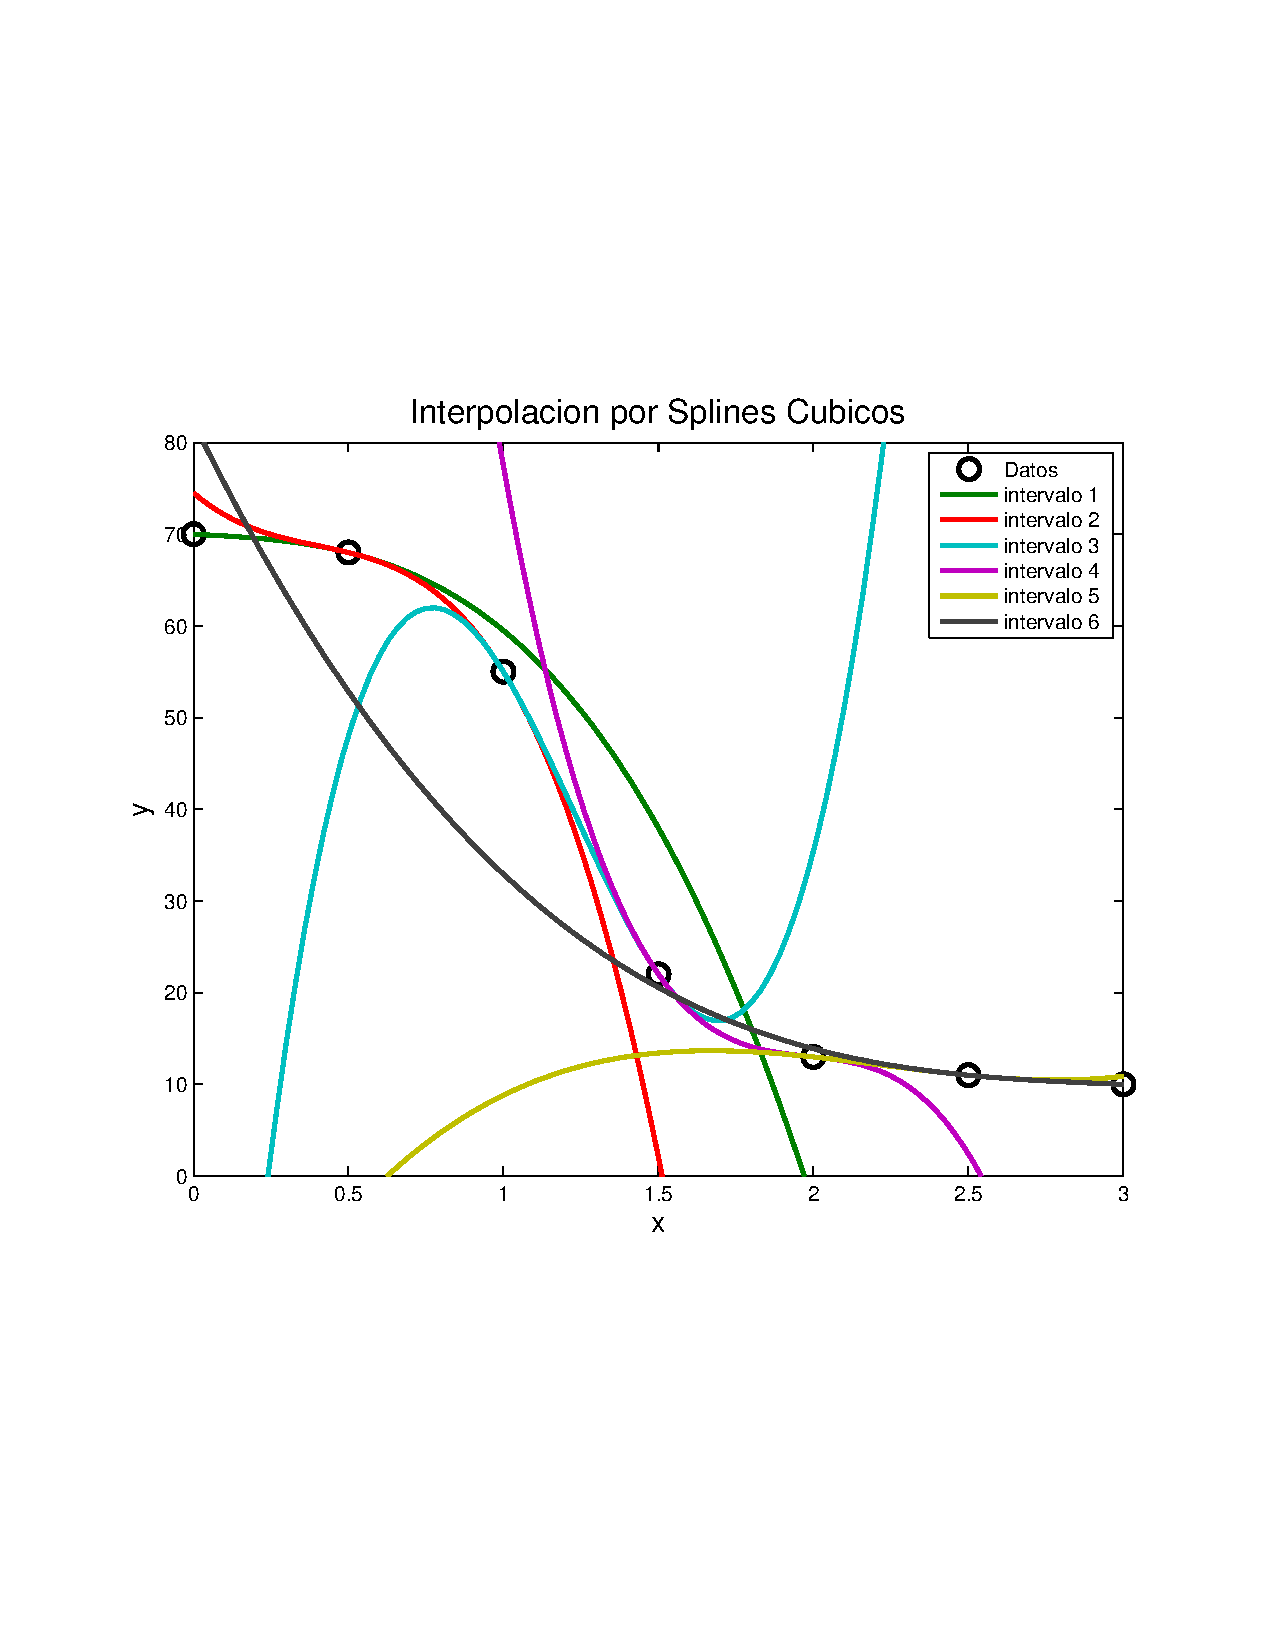
\includegraphics[width=0.6\textwidth,trim=1cm 7cm 1cm 6cm]{./scplines.pdf}
    \caption{\label{FiguraSplinesExtendidos} Cada polinomio vale solo en su intervalo}
  \end{figure}
\end{frame}

\mode<article>
El problema no ha terminado aún. El Enunciado pide, en pocas palabras,
encontrar la profundidad a la que se minimiza la derivada primera
de la función, que será cuando la derivada segunda se anule.
Hay varias maneras de resolver esto. 

En primera instancia, uno podría pensar que la derivada estara bien
representada por la derivada de los polinomios. Esta hipótesis se 
maneja en la \autoref{FiguraDerivPoli}. El problema es que los
polinomios son a lo sumo dos veces derivables, pero lasegunda derivada
si bien es continua es ``aserrada'' de manera que la aproximación
a su cero puede ser tan buena o mala como nuestra tolerancia a
los errores.

\begin{figure}
  \includeslide[width=\textwidth]{FrameFigDerivPoli}
  \caption{\protect\label{FiguraDerivPoli}}
\end{figure}

\mode*
\begin{frame}<presentation>[label=FrameFigDerivPoli]
  \frametitle{Derivar polinomios}
  \center
  \includegraphics[width=0.8\textwidth,page=6,trim=0cm 0cm 0cm 4.1cm,clip]{./Resumen/GUIA1-Resumen-2018.pdf}

\end{frame}

\mode<article>
Otra forma de resolver el problema seria derivar numéricamente los datos
como  se muestra en la \autoref{FigureDerivarDatos}. Notar que con 
este truco se obtienen derivadas suaves, pero las derivadas 
numéricas tienen su error intrínseco y nuevamente es nuestra
tolerancia a los errores la que determinará la confianza que le 
tengamos al resultado. 

no lo hemos dicho, pero el lugar donde se anula la derivada 
segunda podemos encontrarlo usando algún algoritmo 
de optimización. Por ejemplo el método de bisección. 

\begin{figure}
  \includeslide[width=\textwidth]{FrameFigureDerivarDatos}
  \caption{\protect\label{FigureDerivarDatos} Solucion del problema al
  derivar numéricamente los datos}
\end{figure}

\mode*
\begin{frame}<presentation>[label=FrameFigureDerivarDatos]
  \frametitle{Interpolar la derivada numérica de los datos}
  \center
  \includegraphics[width=0.8\textwidth,page=7,trim=0cm 0cm 0cm 4.2cm,clip]{./Resumen/GUIA1-Resumen-2018.pdf}
\end{frame}
>>>>>>> Guia0-Repaso

\mode*
 
\mode<all>




\end{document}
